\documentclass[../main.tex]{subfiles}

\pagestyle{main}
\renewcommand{\chaptermark}[1]{\markboth{\chaptername\ \thechapter\ (#1)}{}}
\renewcommand{\thechapter}{\Roman{chapter}}

\begin{document}




\chapter{Symmetry and Group Theory in Chemistry}
\section{Module 3: Symmetry Elements and Operations}
\begin{itemize}
    \item \marginnote{1/13:}He will upload lecture slides in advance in the future.
    \item An object is symmetric if one part is the same as other parts.
    \item The symmetry of discrete objects is described using \textbf{Point Symmetry}.
    \item \textbf{Point groups} ($\sim 32$ for molecules) provide us with a way to indicate the symmetry unambiguously.
    \item Point groups have symmetry about a single point at the center of mass of the system.
    \item Extended objects (e.g., crystals) have \textbf{translational symmetry} described by \textbf{Space groups}\footnote{Not covered in this course.} (230 total).
    \item Reading: \textcite{bib:MiesslerFischerTarr} Chapter 4 and \url{https://en.wikipedia.org/wiki/Molecular_symmetry}.
    \item \textbf{Symmetry elements}: Geometric entities about which a \textbf{symmetry operation} can be performed. In a point group, all symmetry elements must pass through the center of mass (the point).
    \item \textbf{Symmetry operation}: The action that produces an object identical to the initial object.
\end{itemize}
\begin{tchart}{1.2}{Element}{Operation}
    Identity, $E$ & nothing\\
    Rotation axis, $C_n$ & $n$-fold rotation\\
    Improper rotation axis, $S_n$ & $n$-fold improper rotation\\
    Plane of symmetry, $\sigma$ & Reflection\\
    Center of symmetry, $i$ & Inversion\\
\end{tchart}
\begin{itemize}
    \item \textbf{Identity}: Does nothing to the object, but is necessary for mathematical completeness.
    \item \textbf{$\bm{n}$-fold rotation}: A rotation of $\ang{360}/n$ about the $C_n$ axis ($n\in[1,\infty)$).
    \begin{itemize}
        \item In \ce{H2O}, there is a $C_2$ axis, so we can perform a $2$-fold ($\ang{180}$) rotation to get the same molecule.
        \begin{itemize}
            \item Remember, because of quantum mechanical properties, the hydrogens are indistinguishable so when we rotate it $\ang{180}$, we cannot tell it apart from the unrotated molecule.
        \end{itemize}
        \item Rotations are considered positive in the counterclockwise direction.
        \item Each possible rotation operation is assigned using a superscript integer $m$ of the form ${C_n}^m$. $m$ is the number of sequential applications.
        \item The rotation ${C_n}^n=E$ is equivalent to the identity operation (nothing is moved).
        \item Linear molecules have an infinite number of rotational options $C_\infty$ because any rotation on the molecular axis will give the same arrangement.
    \end{itemize}
    \item \textbf{Principal axis}: The highest order rotation axis.
    \begin{itemize}
        \item By convention, the principal axis is assigned to the $z$-axis if we are using Cartesian coordinates.
    \end{itemize}
    \item \textbf{Reflection}: Exchanges one half of the object with the reflection of the other half.
    \item \textbf{Vertical mirror plane}: A mirror plane that contains the principal axis. \emph{Also known as} $\bm{\sigma_v}$.
    \item \textbf{Horizontal mirror plane}: A mirror plane that is perpendicular to the principal axis. \emph{Also known as} $\bm{\sigma_h}$.
    \item \textbf{Dihedral mirror planes}: A special type of $\sigma_v$ that is between sides or planes. \emph{Also known as} $\bm{\sigma_d}$.
    \begin{itemize}
        \item For example, we might have vertical mirror planes in the $xz$- or $yz$-planes. In this case, the dihedral planes would contain the lines $y=\pm x$.
    \end{itemize}
    \item Two successive reflections are equivalent to the identity operation.
    \item \textbf{Inversion}: Every part of the object is reflected through the inversion center, which must be at the center of mass of the object.
    \begin{itemize}
        \item $(x,y,z)\xrightarrow{i}(-x,-y,-z)$.
    \end{itemize}
    \item \textbf{$\bm{n}$-fold improper rotation}: This operation involves a rotation of $\ang{360}/n$ followed by a reflection perpendicular to the axis. It is a single operation and is labeled in the same manner as "proper" rotations. \emph{Also known as} $\bm{{S_n}^m}$.
    \begin{figure}[h!]
        \centering
        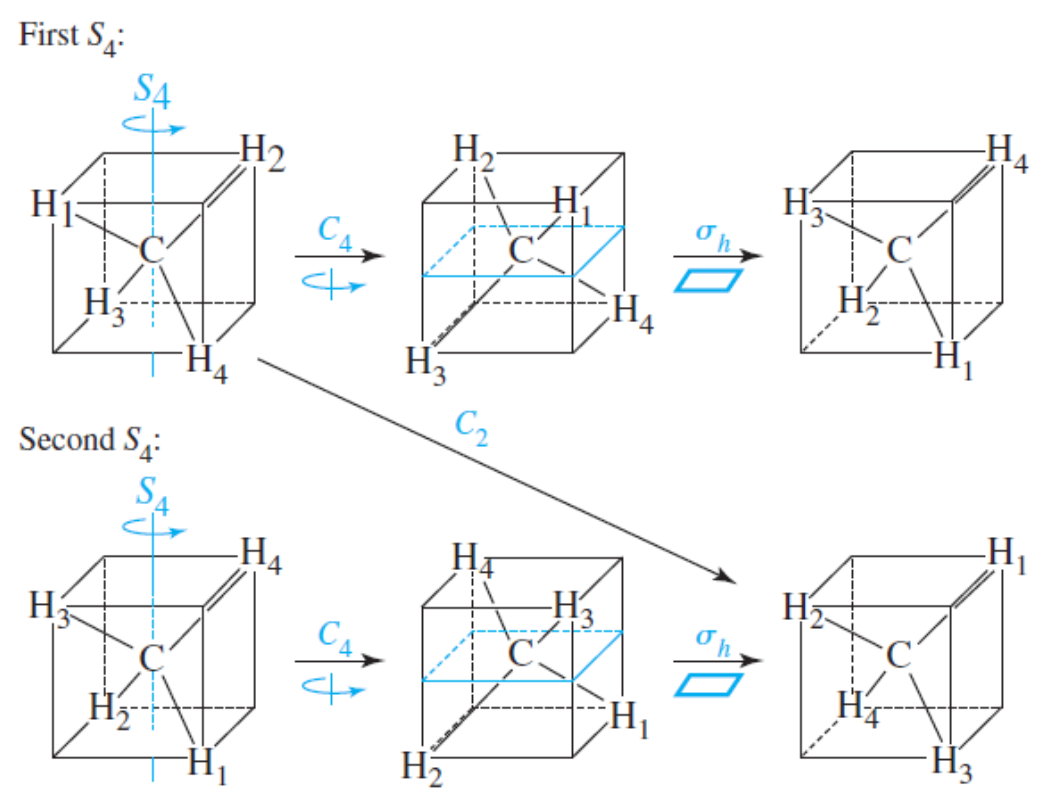
\includegraphics[width=0.4\linewidth]{ExtFiles/methaneImproperRotation.png}
        \caption{Methane's $S_4$ symmetry.}
        \label{fig:methaneImproperRotation}
    \end{figure}
    \begin{itemize}
        \item Methane has $S_4$ symmetry.
        \item Note that $S_1=\sigma_h$, $S_2=i$, and sometimes $S_{2n}=C_n$. In methane, for example, ${S_4}^2=C_2$.
        \item Applied to a triangular prism, is a good example.
        \item If $n$ is even, we have $n$ unique operations. There should be $C_{n/2}$.
        \item If $n$ is odd, we have $2n$ unique operations. There should be $C_n$ and $\sigma_h$.
    \end{itemize}
    \item The absence of an $S_n$ axis is the defining symmetry property of \textbf{chiral} molecules.
    \begin{itemize}
        \item Formerly, we learned that chiral molecules should not have mirror planes and inversion centers.
        \item Rigorously, chiral molecules must not have any improper rotation axes.
    \end{itemize}
\end{itemize}



\section{Module 4: Symmetry Point Groups}
\begin{itemize}
    \item Identifying the point groups:
    \begin{enumerate}
        \item Determine if the symmetry is special (e.g., octahedral).
        \item Determine if there is a principal rotation axis.
        \item Determine if there are rotation axes perpendicular to the principal axis.
        \item Determine if there are mirror planes.
        \item Assign point groups.
    \end{enumerate}
    \item High symmetry and low symmetry groups are the most difficult to identify.
    \item High symmetry:
    \begin{itemize}
        \item Perfect tetrahedral ($T_d$), e.g., \ce{P4} and \ce{CH4}.
        \item Perfect octahedral ($O_h$), e.g., \ce{SF6}.
        \item Perfect icosahedral ($I_h$), e.g., \ce{C60}.
    \end{itemize}
    \item Low symmetry:
    \begin{figure}[h!]
        \centering
        \begin{subfigure}[b]{0.24\linewidth}
            \centering
            \footnotesize
            \chemfig[cram width=3pt,cram dash width=0.5pt,cram dash sep=1.3pt,atom sep=7mm]{*8(<(<[:-120]F_3)=>(>:[:-30]F_2)=<(<[:60]F_1)=>(>:[:150]F_4)=)}
            \caption{$S_4$.}
            \label{fig:lowSymmetrya}
        \end{subfigure}
        \begin{subfigure}[b]{0.24\linewidth}
            \centering
            \footnotesize
            \chemfig{Cl-[1]C(<[:120]H)(>:[:60]F)-[7]Cl}
            \caption{$C_s$}
            \label{fig:lowSymmetryb}
        \end{subfigure}
        \begin{subfigure}[b]{0.24\linewidth}
            \centering
            \footnotesize
            \chemfig{H-[1]C(>:[3]Br)(<[:170]Cl)-C(<[7]Br)(>:[:-10]Cl)-[1]H}
            \caption{$C_i$}
            \label{fig:lowSymmetryc}
        \end{subfigure}
        \begin{subfigure}[b]{0.24\linewidth}
            \centering
            \footnotesize
            \chemfig{C(-[:-30]Br)(<[:-110]Cl)(>:[:-150]F)-[2]H}
            \caption{$C_1$}
            \label{fig:lowSymmetryd}
        \end{subfigure}
        \caption{Low symmetry point groups.}
        \label{fig:lowSymmetry}
    \end{figure}
    \begin{itemize}
        \item Only an improper axis: $S_n$.
        \item Only a mirror plane: $C_s$.
        \item Only an inversion center: $C_i$.
        \item No symmetry: $C_1$.
    \end{itemize}
    \item $C_n$ groups:
    \begin{itemize}
        \item Only a $C_n$ axis. Note that conformation is important.
    \end{itemize}
    \item $C_{nh}$ groups have a $C_n$ axis and a $\sigma_h$ reflection plane (such as \ce{B(OH)3}).
    \begin{itemize}
        \item \ce{H2O2} has $C_{2h}$ symmetry.
    \end{itemize}
    \item All symmetry elements are listed in the top row of the corresponding characters table (Appendix C in \textcite{bib:MiesslerFischerTarr}).
    \item $C_{nv}$ groups have a $C_n$ axis and a $\sigma_v$ reflection plane.
    \begin{itemize}
        \item \ce{NH3} has $C_{3v}$ symmetry.
        \item \ce{CO} has $C_{\infty v}$ symmetry since there are an infinite number of both $C_n$ axes and $\sigma_v$ mirror planes.
    \end{itemize}
    \item $D_{nh}$ groups: A $C_n$ axis, $n$ perpendicular $C_2$ axes, and a $\sigma_h$ reflection plane.
    \begin{itemize}
        \item \ce{BH3} has $D_{3h}$ symmetry.
        \item A square prism has $D_{4h}$ symmetry.
        \item \ce{CO2} has $D_{\infty h}$ symmetry.
    \end{itemize}
    \item $D_n$ groups: A $C_n$ axis, $n$ perpendicular $C_2$ axes, and no mirror planes.
    \begin{itemize}
        \item A 3-bladed propeller has $D_3$ symmetry.
    \end{itemize}
    \item $D_{nd}$ groups: A $C_n$ axis, $n$ perpendicular $C_2$ axes, and a $\sigma_d$.
    \begin{itemize}
        \item Ethane in the staggered conformation has $D_{3d}$ symmetry.
    \end{itemize}
    \item Local symmetry:
    \begin{itemize}
        \item Sometimes, rigorous math analysis needs to be adjusted to physical reality.
        \item If a cyclopentane ring is bonded through the center to \ce{Mn(CO)3}, this molecule has only $C_s$ symmetry.
        \item However, spectroscopically, there is fast rotation about the \ce{Mn-Cp} bond. This means that the \ce{Mn(CO)3} fragment exhibits pseudo-$C_{3v}$ symmetry while the \ce{C5H5} ligand exhibits pseudo-$C_{5v}$ symmetry.
        \item Often, the absolute symmetry of a molecule is very low, but the interactions are far away from the centers of interest, and do not perturb them significantly.
        \item If we have platinum as a central atom bonded to two chlorines and two \ce{P(Et)3} groups, this molecule technically has $C_1$ symmetry due to the orientations of atoms within \ce{R} groups (staggered), but IR spectroscopy is characteristic of highly symmetric species ($D_{2h}$).
    \end{itemize}
\end{itemize}



\section{Module 5: Group Theory 101}
\begin{itemize}
    \item \marginnote{1/15:}\textbf{Group}: A set of elements together with an operation that combines any two of its elements to form a third element satisfying four conditions called the group axioms.
    \item \textbf{Closure}: All binary products must be members of the group.
    \item \textbf{Associativity}: Associative law of multiplication must hold.
    \item \textbf{Identity}: A group must contain the identity operator.
    \item \textbf{Inverse}: Every operator must have an inverse.
    \item The integers with the addition operation form a group, for example.
    \item History:
    \begin{itemize}
        \item Early group theory was driven by the quest for solutions of polynomial equations of degree 5 and above.
        \item Early 1800s: \'{E}variste Galois realized that the algebraic solution to a polynomial equation is related to the structure of a group of permutations associated with the roots off the polynomial, the Galois group of the polynomial.
        \begin{itemize}
            \item Link to Galois video \href{https://www.youtube.com/watch?v=Ct2fyigNgPY}{here}.
        \end{itemize}
        \item 1920s: Group theory was applied to physics and chemistry.
        \item 1931: It is often hard or even impossible to obtain a solution of the Schr\"{o}dinger equation --- however, a large part of qualitative results can be obtained by group theory. Almost all the rules of spectroscopy follow from the symmetry of a problem.
    \end{itemize}
    \item We will use group theory for describing symmetry of molecules. We will use group theory to understand the bonding and spectroscopic features of molecules.
    \item For us, a group consists of a set of symmetry elements (and associated symmetry operations) that completely describes the symmetry of a molecule.
    \item \textbf{Order} (of a group): The total number of elements (i.e., symmetry operations) in the group. \emph{Also known as} $\bm{h}$.
    \item Rule 1: Closure.
    \begin{figure}[h!]
        \centering
        \begin{tikzpicture}
            \footnotesize
            \fill [orange!80!yellow,opacity=0.2] (-2,-1.2) rectangle (2,1.4) node[black,opacity=1,right]{$\sigma_v'$};
            \fill [orange!50!yellow,opacity=0.35] (0,-1.2,-2) -- (0,1.4,-2) -- (0,1.4,2) -- (0,-1.2,2) node[black,opacity=1,right]{$\sigma_v$};
            \draw [very thick,-stealth] (0,1.4,0) -- (0,3,0) node[above]{$z$};
            \draw [yshift=2cm,very thick,arrows={->[scale width=0.6,flex=2]}] (-120:0.3cm and 0.1cm) arc[start angle=240,end angle=-70,x radius=0.3cm,y radius=0.1cm] node[xshift=-7mm,yshift=1mm]{$C_2$};
    
            \draw [thick] (-1,-0.6) node[circle,ball color=gray]{} node[below=1mm]{1} -- (0,0) node[circle,ball color=red,inner sep=5pt]{} -- (1,-0.6) node[circle,ball color=gray]{} node[below=1mm]{2};
    
            \draw [very thick,-stealth] (0.25,0,0) -- (1,0,0) node[right]{$y$};
            \draw [very thick,-stealth] (0,0.25,0) -- (0,1,0) node[above]{$z$};
            \draw [very thick,-stealth] (0,0,0.25) -- (0,0,1.3) node[below left=-1mm]{$x$};
        \end{tikzpicture}
        \caption{Symmetry elements for \ce{H2O}.}
        \label{fig:symmetry-H2O}
    \end{figure}
    \begin{itemize}
        \item \ce{H2O} is of the $C_{2v}$ point group (refer to Figure \ref{fig:symmetry-H2O}).
        \begin{itemize}
            \item Symmetry operations: $E$, $C_2$, $\sigma_{v(xz)}$, and $\sigma'_{v(yz)}$.
            \item $\sigma_v\cdot C_2=\sigma_v'=C_2\cdot\sigma_v$.
            \item The above property (order \emph{does not} matter) shows that $C_{2v}$ is an \textbf{Abelian group}.
        \end{itemize}
        \item \ce{NH3} is of the $C_{2v}$ point group.
        \begin{itemize}
            \item Symmetry operations: $E$, ${C_3}^+$, ${C_3}^-$, $\sigma_v$, $\sigma_v'$, and $\sigma_v''$.
            \item $\sigma_v''\cdot C_3=\sigma_v$, but $C_3\cdot\sigma_v''={C_3}^-={C_3}^2$.
            \item The above property (order \emph{does} matter) shows that $C_{3v}$ is a \textbf{non-Abelian group}.
        \end{itemize}
    \end{itemize}
    \item Rule 2: Associativity.
    \begin{itemize}
        \item \ce{H2O} is of the $C_{2v}$ point group (refer to Figure \ref{fig:symmetry-H2O}).
        \begin{align*}
            \sigma_v'C_2\sigma_v(1,2) &= \sigma_v'C_2(2,1)&
                \sigma_v'(C_2\sigma_v)(1,2) &= \sigma_v'E(1,2)&
                    (\sigma_v'C_2)\sigma_v(1,2) &= \sigma_v\sigma_v(1,2)\\
            &= \sigma_v'(1,2)&
                &= \sigma_v'(1,2)&
                    &= \sigma_v(2,1)\\
            &= (1,2)&
                &= (1,2)&
                    &= (1,2)
        \end{align*}
    \end{itemize}
    \item Rule 3: Identity.
    \item Rule 4: Inverse.
    \begin{itemize}
        \item For a $C_{2v}$ point group:
        \begin{align*}
            E\cdot E &= E&
            C_2\cdot C_2 &= E&
            \sigma_v\cdot\sigma_v &= E&
            \sigma_v'\cdot\sigma_v' &= E
        \end{align*}
    \end{itemize}
    \item Group multiplication tables.
    \begin{table}[H]
        \centering
        \renewcommand{\arraystretch}{1.4}
        \footnotesize
        \begin{tabular}{l|llll}
            \normalsize$C_{2h}$ & $\bm{E}$   & $\bm{C_2}$ & $\bm{\sigma_h}$ & $\bm{i}$\\
            \hline
            $\bm{E}$            & $E$        & $C_2$      & $\sigma_h$      & $i$\\
            $\bm{C_2}$          & $C_2$      & $E$        & $i$             & $\sigma_h$\\
            $\bm{\sigma_h}$     & $\sigma_h$ & $i$        & $E$             & $C_2$\\
            $\bm{i}$            & $i$        & $\sigma_h$ & $C_2$           & $E$\\
        \end{tabular}
        \caption{Group multiplication table for the $C_{2h}$ point group.}
        \label{tab:groupMultiplication-C2h}
    \end{table}
    \begin{itemize}
        \item Table \ref{tab:groupMultiplication-C2h} corresponds to the $C_{2h}$ point group, which has $E$, $C_2$, $\sigma_h$, and $i$ operations.
        \item Note that the operation in the top row is the one that's applied first, while the one in the left column will be applied second.
    \end{itemize}
    \item \textbf{Subgroup}: Fractional parts of groups that are groups, too.
    \begin{table}[h!]
        \centering
        \renewcommand{\arraystretch}{1.4}
        \footnotesize
        \begin{tabular}{l|llllll}
            \normalsize$C_{2v}$ & $\bm{E}$ & $\bm{C_3}$ & $\bm{{C_3}^2}$ & $\bm{\sigma_v}$ & $\bm{\sigma_v'}$ & $\bm{\sigma_v''}$\\
            \hline
            $\bm{E}$            & $E$ & $C_3$ & ${C_3}^2$ & $\sigma_v$ & $\sigma_v'$ & $\sigma_v''$\\
            $\bm{C_3}$          & $C_3$ & ${C_3}^2$ & $E$ & $\sigma_v''$ & $\sigma_v$ & $\sigma_v'$\\
            $\bm{{C_3}^2}$      & ${C_3}^2$ & $E$ & $C_3$ & $\sigma_v'$ & $\sigma_v''$ & $\sigma_v$\\
            $\bm{\sigma_v}$     & $\sigma_v$ & $\sigma_v'$ & $\sigma_v''$ & $E$ & $C_3$ & ${C_3}^2$\\
            $\bm{\sigma_v'}$    & $\sigma_v''$ & $\sigma_v$ & $\sigma_v'$ & $C_3$ & ${C_3}^2$ & $E$\\
            $\bm{\sigma_v''}$   & $\sigma_v'$ & $\sigma_v''$ & $\sigma_v$ & ${C_3}^2$ & $E$ & $C_3$\\
        \end{tabular}
        \begin{tikzpicture}[remember picture,overlay]
            \draw [red,thick] (-6.75,1.73) rectangle (-4.9,0.75);
            \draw [blue,thick] (-6.78,1.76) rectangle (-3.9,0.3);
            \draw [red!50!blue,thick] (-6.81,1.79) rectangle (-2.9,-0.15);
        \end{tikzpicture}
        \caption{Group multiplication table for the $C_{2v}$ point group.}
        \label{fig:groupMultiplication-C2v}
    \end{table}
    \begin{itemize}
        \item If $h=6$ (as in the $C_{3v}$ group), subgroup order can be $h={\color{red!50!blue}3},{\color{blue}2},{\color{red}1}$. Why only these?
        \item The order ${\color{red}1}$ and ${\color{red!50!blue}3}$ charts are subgroups.
        \item The order ${\color{blue}2}$ chart is not a subgroup because ${C_3}^2$ is not an operation in the group (therefore, the "subgroup" is not closed).
    \end{itemize}
    \item We use subgroups because they can make complex problems simpler.
    \begin{itemize}
        \item For example, calculating the vibrational modes of \ce{CO2}.
        \item As another example, $D_{2h}$ is a subgroup of $D_{\infty h}$.
    \end{itemize}
\end{itemize}



\section{Module 6: Representations}
\begin{itemize}
    \item Items of the same point group have the same vibration modes.
    \item \textbf{Representation} (of a group): Any collection of quantities (or symbols) which obey the multiplication tabble of a group. \emph{Also known as} $\Gamma$.
    \item For our purposes, these quantities are the matrices that show how certain characteristic of a molecule behave under the symmetry operations of the group.
    \item Operations (on a point $(x,y,z)$ in Cartesian coordinates):
    \begin{itemize}
        \item $E(x,y,z)=(x,y,z)$.
        \item $\sigma_{xz}(x,y,z)=(x,-y,z)$.
        \item $i(x,y,z)=(-x,-y,-z)$.
        \item $C_n$: Convention is a counterclockwise rotation of the point by $\theta=\frac{2\pi}{n}$ radians.
        \item $S_n$: Convention is a clockwise rotation of the point $C_n$ followed by a $\sigma$ through a plane perpendicular to $C$.
    \end{itemize}
    \item Matrix forms of operations:
    \begin{itemize}
        \item Identity: $
            E =
            \begin{bmatrix}
                1 & 0 & 0\\
                0 & 1 & 0\\
                0 & 0 & 1\\
            \end{bmatrix}
        $.
        \item One example of a reflection (there are two more): $
            \sigma_{xy} =
            \begin{bmatrix}
                1 & 0 & 0\\
                0 & 1 & 0\\
                0 & 0 & -1\\
            \end{bmatrix}
        $.
        \item Inversion: $
            i =
            \begin{bmatrix}
                -1 & 0 & 0\\
                0 & -1 & 0\\
                0 & 0 & -1\\
            \end{bmatrix}
        $.
        \item Rotation: Counterclockwise is $
            C_n(\theta) =
            \begin{bmatrix}
                \cos\theta & -\sin\theta & 0\\
                \sin\theta & \cos\theta & 0\\
                0 & 0 & 1\\
            \end{bmatrix}
        $ and clockwise is $
            C_n(\theta) =
            \begin{bmatrix}
                \cos\theta & \sin\theta & 0\\
                -\sin\theta & \cos\theta & 0\\
                0 & 0 & 1\\
            \end{bmatrix}
        $.
        \begin{itemize}
            \item A derivation of this matrix can be found in the slides.
        \end{itemize}
        \item Improper rotation: $S_n(\theta)=\sigma_hC_n(\theta)$.
    \end{itemize}
    \item \textbf{Reducible representations}:
    \begin{itemize}
        \item A representation of a symmetry operation of a group.
        \item Can be expressed in terms of a representation of lower dimension.
        \item Can be broken down into a simpler form.
        \item Characters can be further diagonalized.
        \item Are composed of the direct sum of irreducible representations.
        \item Infinite possibilities.
    \end{itemize}
    \item \textbf{Irreducible representations}:
    \begin{itemize}
        \item A fundamental representation of a symmetry operation of a group.
        \item Cannot be expressed in terms of a representation of lower dimension.
        \item Cannot be broken down into a simpler form.
        \item Characters cannot be further diagonalized.
        \item Small finite number dictated by point group.
    \end{itemize}
    \item Good example of reducible/irreducible representations?
\end{itemize}




\end{document}